\section{Técnicas de Deep Learning y métodos de evaluación}
\label{sec:tecnicas_de_deep_learning_y_metodos_de_evaluacion}

\subsection{Explicar las técnicas de DL que se van a utilizar en el proyecto}

A continuación se explicarán las principales técnicas utilizadas para el desarrollo del proyecto. Algunas de las técnicas mencionada no son específicas del deep learning.

La primera de las técnicas es una de las técnicas \textit{generalistas}, propia de los algoritmos de aprendizaje en general. Se trata del \textit{hold-out}, que consiste en dividir el conjunto de datos en dos subconjuntos: uno que se utiliza para el entrenamiento y otro que se utiliza para evaluar el modelo obtenido tras el entrenamiento.

Para el desarrollo del proyecto se ha implementado una \textit{red neuronal convolucional (CNN)} \cite{s5_cnn1} \cite{s5_cnn2} \cite{s5_cnn3}. Las \textit{CNNs} están compuestas por una secuencia de capas convolucionales, para la extracción de características, seguidas de unas capas perceptrón simples, para la clasificación final. Las capas convolucionales forman una jerarquía, de forma que las capas del principio son capaces de detectar formas básicas y cuanto más ``profunda'' es la capa, más complejas son las formas que son capaces de detectar. Por ejemplo: una capa inicial sería capaz de detectar líneas y círculos, mientras que una capa profunda sería capaz de detectar una cara.

Las capas convolucionales están compuestas por neuronas que realizan la operación de \textit{convolución}. Dichas neuronas reciben en la entrada una matriz bidimensional, que se corresponde con la imagen, si se trata de la primera capa de la red, o con la salida de la capa convolucional anterior. Además, cada una de estas neuronas tiene definido un \textit{kernel}, que es otra matriz bidimensional de dimensiones reducidas.

\begin{figure}[H]
	\centering
	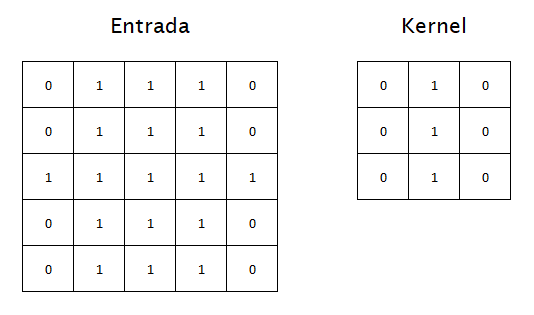
\includegraphics[width=0.7\linewidth]{images/convolutional_neuron_example.png}
	\caption{Ejemplo de neurona convolucional con una entrada de 5x5 y un kernel de 3x3}
	\label{fig:cnn_neuronex}
\end{figure}

La operación de \textit{convolución} consiste en hacer un barrido del \textit{kernel} por la matriz de entrada, de izquierda a derecha y de arriba a abajo. En cada una de las posiciones del barrido se aplica el producto escalar entre el kernel y la submatriz de la matriz de entrada sobre la que se encuentre. En la figura \ref{fig:cnn_convolutionoperationex} se puede ver gráficamente el proceso.

\begin{figure}[H]
	\centering
	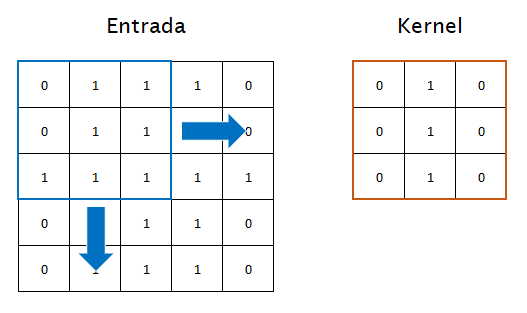
\includegraphics[width=0.7\linewidth]{images/convolutional_operation_example.png}
	\caption{Representación gráfica de operación convolucional}
	\label{fig:cnn_convolutionoperationex}
\end{figure}

Para realizar el producto escalar, las matrices se \textit{aplanan}, de tal forma que la submatriz de entrada quedaría de la siguiente forma:

\begin{equation}
	\left[
	\begin{array}{ccc}
		0 & 1 & 1 \\
		0 & 1 & 1 \\
		0 & 1 & 1 \\
	\end{array}
	\right]
	=>
	\left[
	\begin{array}{ccccccccc}
		0 & 1 & 1 & 0 & 1 & 1 & 0 & 1 & 1 \\
	\end{array}
	\right]
	\nonumber
\end{equation}

El kernel:

\begin{equation}
	\left[
	\begin{array}{ccc}
		0 & 1 & 0 \\
		0 & 1 & 0 \\
		0 & 1 & 0 \\
	\end{array}
	\right]
	=>
	\left[
	\begin{array}{ccccccccc}
		0 & 1 & 0 & 0 & 1 & 0 & 0 & 1 & 0 \\
	\end{array}
	\right]
	\nonumber
\end{equation}

Y por lo tanto el producto escalar:

\begin{equation}
	\left[
	\begin{array}{ccccccccc}
		0 & 1 & 1 & 0 & 1 & 1 & 0 & 1 & 1 \\
	\end{array}
	\right]
	\left[
	\begin{array}{c}
		0 \\
		1 \\
		0 \\
		0 \\
		1 \\
		0 \\
		0 \\
		1 \\
		0 \\
	\end{array}
	\right] = 3
	\nonumber
\end{equation}

Cada una de las neuronas de las capas convolucionales no tiene un único kernel asociado, sino que tienen varios. Teniendo en cuenta esto y suponiendo que tenemos como entrada una imagen en blanco y negro de $28x28$ píxeles y que cada neurona tiene $32$ kernels de $3x3$, la primera capa convolucional estaría compuesta por $28 x 28 = 784$ neuronas, y se obtendrían como resultado $28 x 28 x 32 = 25.088$ matrices de salida, que se correspondería con el número de neuronas necesarias para la siguiente capa convolucional. Esto hace necesario introducir un mecanismo de reducción para que el número de neuronas necesarias no crezca tan desmesuradamente con cada capa. Este mecanismo se conoce como \textit{pooling} y existen distintos tipos de pooling. Uno de ellos es el \textit{MaxPooling}, y consiste en deslizar una ventana bidimensional sobre la matriz de entrada, de izquierda a derecha y de arriba a abajo. En cada una de las posiciones se tomará como valor resultante el máximo valor presente en la ventana. La capacidad de reducción del MaxPooling depende de dos factores: el tamaño de la ventana y el tamaño del salto que se da hacia la derecha y hacia abajo. En la figura \ref{fig:cnn_maxpooling} se muestra un ejemplo gráfico.

\begin{figure}[H]
	\centering
	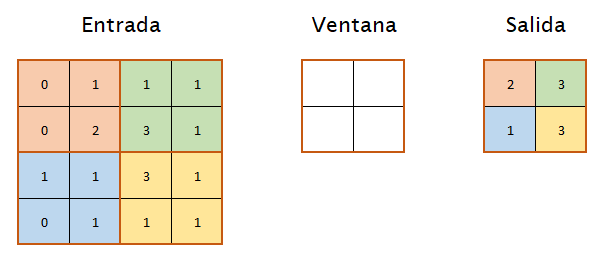
\includegraphics[width=0.7\linewidth]{images/maxpooling_example.png}
	\caption{Representación gráfica de MaxPooling con una entrada de 4x4, una ventana de 2x2 y un salto de 2}
	\label{fig:cnn_maxpooling}
\end{figure}

Las redes neuronales convolucionales utilizadas para la detección de objetos tienen como entrada una matriz bidimensional que se corresponde con la imagen (en caso de ser una imagen a color, serán 3 matrices bidimensionales, una por cada canal de color). Como salida se obtiene una lista de predicciones, cada una de las cuales se compone de una región representada por cuatro variables (coordenadas x e y de la esquina superior izquierda, anchura y altura) y de las probabilidades pertencencia del objeto en la región a cada una de las clases que la red es capaz de predecir.

Otra de las técnicas que se han utilizado en el proyecto es la denominada \textit{transferencia del conocimiento (transfer learning)} \cite{s5_transfer_learning}. Entrenar un modelo de detección de objetos es un proceso muy costoso, ya que se necesita un gran volumen de imágenes y una gran capacidad de cómputo. El \textit{transfer learning} viene a paliar este problema ya que permite utilizar un modelo ya entrenado como punto de partida para entrenar otro. Como se ha comentado anteriormente, las primeras capas convolucionales son capaces de detectar formas básicas y a medida que se profundiza en las capas, estas detectan formas más específicas. Si ya tenemos entrenado un modelo (a) para detectar un determinado tipo de objetos y queremos entrenar otro (b) para detectar otro tipo de objetos, las primeras capas de ambos modelos van a detectar el mismo tipo de formas, y serán las capas más profundas las que se diferencien. Por lo tanto podríamos utilizar el modelo \textit{a} como punto de partida para el modelo \textit{b}, y este último podrá aprender más rápido ya que las primeras capas ya están entrenadas para detectar formas básicas.

\subsection{Explicar los métodos de evaluación que se van a utilizar en el proyecto}

La métrica que se ha utilizado para evaluar el modelo obtenido es la \textit{AP} (Average Precision), que es la métrica que se utiliza para evaluar modelos de detección de objetos.

Antes de explicar en qué consiste la métrica \textit{AP} hay que explicar una serie de conceptos en los cuales está basada: IoU (intersección sobre la unión), precisión (precision) y sensibilidad (recall).

El concepto de \textit{IoU} mide cuánto se solapan dos regiones: la predicha y la que debería ser detectada. Se calcula dividiendo la región obtenida mediante la intersección de la región predicha y la región a detectar entre la región obtenida mediante la unión de ambas regiones.

\begin{equation}
	AP = \frac{interseci\acute{o}n}{uni\acute{o}n} = \frac{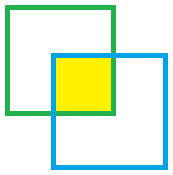
\includegraphics[width=0.2\linewidth]{images/ap_intersection.png}}{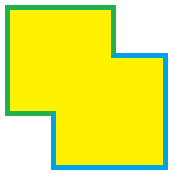
\includegraphics[width=0.2\linewidth]{images/ap_union.png}}
	\nonumber
\end{equation}

La \textit{precisión} (precision) mide la capacidad del modelo para detectar únicamente los objetos relevantes. Se calcula como el porcentaje de predicciones positivas acertadas frente a todas las predicciones positivas predichas:

\begin{equation}
	precisi\acute{o}n = \frac{TP}{TP + FP} = \frac{TP}{todas\ las\ predicciones\ positivas}
	\nonumber
\end{equation}

La \textit{sensibilidad} (recall)  mide la capacidad del modelo para detectar todos los objetos relevantes. Se calcula como el porcentaje de predicciones positivas acertadas frente a todas las existentes:

\begin{equation}
	sensibilidad = \frac{TP}{TP + FN} = \frac{TP}{todas\ las\ regiones\ a\ detectar}
	\nonumber
\end{equation}

Tanto en el cálculo de la \textit{precisión} como en el cálculo de la \textit{sensibilidad}, para determinar si una predicción es positiva, se utiliza el \textit{IoU}. Se define un umbral para el \textit{IoU} (normalmente suele ser 0.5) y si se supera dicho umbral, la predicción es considerada una predicción positiva.

La métrica \textit{AP} se calcula como el área debajo de la curva \textit{precisión-sensibilidad} (precision-recall). En el eje de las abscisas se representa la \textit{sensibilidad} (recall) y en el eje de las ordenadas se representa la \textit{precisión} (precision).

A continuación se va a mostrar un ejemplo práctico de cómo se calcula la \textit{AP}. Para este ejemplo se dispone de una serie de imágenes con un total de 4 baches a detectar. En la tabla \ref{tab:apprecisionrecalltable} se puede ver el cálculo de la \textit{precisión} y de la \textit{sensibilidad} para las predicciones obtenidas. La columna \textit{Positivo} indica si la predicción es positiva, es decir, si el valor de \textit{IoU} supera el umbral definido, que en este caso es 0.5. Las columnas \textit{TP} y \textit{FP} muestran el acumulado de sus respectivos valores.

\begin{table}[H]
	\centering
	\begin{tabular}{rrrrrr}
		\toprule
		IoU &  Positivo &  TP &  FP &  Precisión &  Sensibilidad \\
		\midrule
		0.912933 &         1 &   1 &   0 &   1.000000 &          0.25 \\
		0.711111 &         1 &   2 &   0 &   1.000000 &          0.50 \\
		0.387983 &         0 &   2 &   1 &   0.666667 &          0.50 \\
		0.387983 &         0 &   2 &   2 &   0.500000 &          0.50 \\
		0.387983 &         0 &   2 &   3 &   0.400000 &          0.50 \\
		1.000000 &         1 &   3 &   3 &   0.500000 &          0.75 \\
		0.225986 &         0 &   3 &   4 &   0.428571 &          0.75 \\
		0.225986 &         0 &   3 &   5 &   0.375000 &          0.75 \\
		1.000000 &         1 &   4 &   5 &   0.444444 &          1.00 \\
		\bottomrule
	\end{tabular}
	\caption{Cálculo de la precisión y sensibilidad para las predicciones}
	\label{tab:apprecisionrecalltable}
\end{table}

Una vez se tienen calculados los valores de \textit{precisión} y de \textit{sensibilidad} se calcula la curva \textit{precisión-sensibilidad} como se puede ver en la figura \ref{fig:apprecisionrecallcurve}. Para realizar el cálculo del área debajo de la curva se realiza un suavizado de la misma. Este suavizado consiste en establecer como valor de \textit{precisión} para un determinado valor de \textit{sensibilidad}, el valor de \textit{precisión} más alto que se encuentre a su derecha. Por ejemplo, para la \textit{sensibilidad} 0.6 se establece como valor de \textit{precisión} el valor más alto a su derecha, que en este caso es 0.5. En color naranja se puede ver la curva suavizada.

\begin{figure}[H]
	\centering
	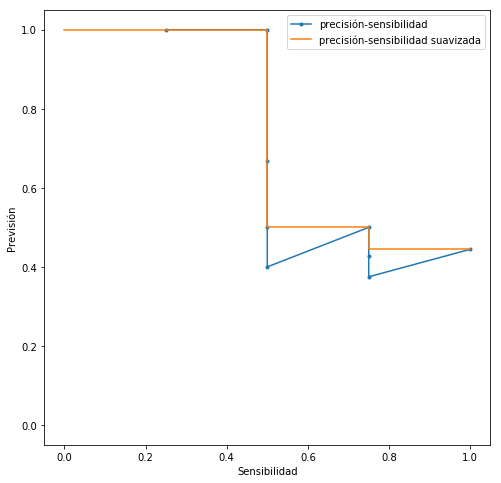
\includegraphics[width=0.7\linewidth]{images/ap_precision_recall_curve.png}
	\caption{Curva precisión-sensibilidad}
	\label{fig:apprecisionrecallcurve}
\end{figure}

Por lo que finalmente, para este ejemplo, el cálculo del \textit{AP} sería:

\begin{equation}
	AP = (0.5 - 0) \cdot 1 + (0.75 - 0.5) \cdot 0.5 + (1 - 0.75) \cdot 0.44 = 0.5 + 0.125 + 0.11 = \textbf{0.735}
	\nonumber
\end{equation}